%\documentclass{beamer}
\documentclass[a4paper]{article}
% \documentclass[10pt]{article}

\usepackage{float}
\usepackage{ctex}
\usepackage{graphicx} 
\usepackage{geometry}
\usepackage{tikz}
\usepackage{amsmath}
\usepackage{setspace}
\usepackage{subcaption}
% for table
\usepackage{tabularx}

%引入python/matlab包
\usepackage{listings}
\usepackage{color}
\definecolor{dkgreen}{rgb}{0,0.6,0}
\definecolor{gray}{rgb}{0.5,0.5,0.5}
\definecolor{mauve}{rgb}{0.58,0,0.82}
\lstset{frame=tb,
  language=Python,
  aboveskip=3mm,
  belowskip=3mm,
  showstringspaces=false,
  columns=flexible,
  basicstyle={\small\ttfamily},
  numbers=left,%设置行号位置none不显示行号
  %numberstyle=\tiny\courier, %设置行号大小
  numberstyle=\tiny\color{gray},
  keywordstyle=\color{blue},
  commentstyle=\color{dkgreen},
  stringstyle=\color{mauve},
  breaklines=true,
  breakatwhitespace=true,
  escapeinside=``,%逃逸字符(1左面的键),用于显示中文例如在代码中`中文...`
  tabsize=4,
  extendedchars=false %解决代码跨页时,章节标题,页眉等汉字不显示的问题
}


\definecolor{mygreen}{rgb}{0,0.6,0}
\definecolor{mygray}{rgb}{0.5,0.5,0.5}
\definecolor{mymauve}{rgb}{0.58,0,0.82}



\usetikzlibrary{positioning, shapes.geometric}
%\usepackage[english, chinese]{babel}

% \usepackage{polyglossia}
% \setmainlanguage{english}
% \setotherlanguage{chinese}
%设置段间距
\setlength{\parskip}{1em}
%设置行间距
\renewcommand{\baselinestretch}{1.5}


\geometry{left=2.54cm, right=2.54cm, top=3.18cm, bottom=3.18cm}
\graphicspath{{./figures/}}
%\newcommand{\myud}{\textbf{}}

\title{Unified Vision-Language Pre-Training for Image Captioning and VQA}
\author{LoongCat}
\date{\today}

\begin{document}
\begin{sloppypar}
      \maketitle
      \newpage
      \begin{spacing}{1}
            %\tableofcontents
            {\small \tableofcontents}
      \end{spacing}


      \newpage



      \section{Abstract}

      本文介绍了一种统一的视觉语言预训练(VLP)模型。该模型的统一性表现在:

      \begin{enumerate}
            \item 它可以针对视觉语言生成(例如图像描述)或理解(例如视觉问答)任务进行微调
            \item 它使用了一个共享的多层Transformer网络进行编码和解码
      \end{enumerate}

      许多现有方法不同使用分离的模型实现编码器和解码器。

      统一的VLP模型使用无监督学习目标对大量图像文本对进行预训练,这两个任务是双向(Bidirectional)和序列到序列(seq2seq)掩码视觉语言预测。这两个任务的不同之处仅在于预测条件所在的上下文。这是通过利用特定的自注意力掩码来控制共享Transformer网络实现的.

      据我们所知,VLP是第一个在图像描述和视觉问答等截然不同的视觉语言生成和理解任务上均取得最先进结果的模型,在三个具有挑战性的基准数据集上(COCO Captions、Flickr30k Captions和VQA 2.0)都表现出色。代码和预训练模型可在https://github.com/LuoweiZhou/VLP找到。
      \section{Introduction}

      %一些值得思考的东西:
      \begin{itemize}
            \item bidirectional and sequence to sequence (seq2seq) masked language prediction是什么
                  \begin{itemize}
                        \item 双向(Bidirectional)预测:
                              在双向预测任务中,模型需要根据给定的上下文信息,预测当前位置的词语或标记。这种预测是"双向"的,因为模型考虑了当前位置左侧和右侧的上下文信息。在处理序列数据时,模型可以同时利用当前位置的左侧和右侧的信息,以便更准确地进行预测。

                        \item 序列到序列(seq2seq)预测:
                              序列到序列预测任务涉及将一个输入序列映射到一个输出序列。这种任务通常用于机器翻译、文本摘要、对话生成等任务中。在序列到序列的模型中,通常包括一个编码器(用于处理输入序列并生成上下文表示)和一个解码器(用于基于编码器的上下文表示生成输出序列)。
                  \end{itemize}
            \item 只有encoder的模型的优缺点?en-de模型对比单en的好处?

                  decoder-only:把输入的内容看成自己已经生成的内容,基于已经生成的内容再去生成

                  %CBOW?用其他词去合成目标词

                  %skip-gram?
      \end{itemize}



      目前模型大多基于BERT,采用两阶段的训练方案:
      \begin{itemize}
            \item 预训练 :在大量图像文本对上基于他们的内模态或扩模态关系预测屏蔽单词或图像区域,学习上下文化的视觉语言表示
            \item 微调   :用于下游任务
      \end{itemize}


      针对不同任务有不同的模型,此外,有许多模型只训练了encoder,并没有对decoder做预训练,会导致encoder的输出与decoder所需要的输入有差异。因此要训练一个统一的编码、解码表示。


      提出的VLP与基于BERT的模型相比有两个主要优势:
      \begin{enumerate}
            \item VLP统一了编码器和解码器,学习了更通用的上下文化视觉语言表示,可以更容易地进行视觉语言生成和理解任务的微调,如图像描述和VQA等
            \item 统一的预训练流程为两种不同的视觉语言预测任务提供了单一的模型架构,即双向和序列到序列,减轻了不同类型任务的多个预训练模型的需求,而不会在任务特定指标上产生显著的性能损失
      \end{enumerate}


      \begin{table*}[!htbp]
            \renewcommand\arraystretch{2}

            \centering
            %\caption{A table with line breaks}
            \begin{tabularx}{\textwidth}{|X|}
                  \hline
                  统一了编码器与解码器,怎么统一的? \\
                  \hline
            \end{tabularx}%

      \end{table*}%

      我们在图像描述和VQA任务上使用了三个具有挑战性的基准数据集(COCO Captions,Flickr30k Captions和VQA 2.0数据集)对VLP进行了验证。我们观察到,与不使用任何预训练模型或仅使用预训练语言模型(即BERT)的两种情况相比,使用VLP显著加快了任务特定的微调速度,并导致更好的任务特定模型,如图1所示。更重要的是,我们的模型在所有三个数据集上都取得了最先进的结果,而没有任何花哨的技巧。


      \section{Related works}

      Language  Pretraining : 在语言预训练的众多BERT变种中,我们回顾了两种与我们方法最相关的方法,即Unified LM或UniLM(Dong等,2019年)和Multi-Task DNN(MTDNN)(Liu等,2019a年)。UniLM采用共享的Transformer网络,在三个语言建模目标上进行预训练:单向、双向和序列到序列。每个目标通过在自注意力掩码中指定不同的二进制值来控制语言模型可以访问的上下文。MT-DNN将多任务训练和预训练相结合,通过将任务特定的投影头附加到BERT网络上。我们的工作受到了这些工作的启发,特别是针对视觉语言任务进行了定制。
      \begin{table*}[!htbp]
            \renewcommand\arraystretch{2}

            \centering
            %\caption{A table with line breaks}
            \begin{tabularx}{\textwidth}{|X|}
                  \hline
                  什么是共享的Transformer网络?
                  \\
                  \hline
            \end{tabularx}%

      \end{table*}%

      %Vision-Language Pre-training  : 这已经成为视觉语言社区中一个新兴的研究领域。相关工作包括ViLBERT(Lu等,2019年)和LXMERT(Tan和Bansal,2019年),它们都仅处理基于理解的任务(例如,VQA和检索),并共享相同的双流BERT框架,其中包含一个视觉语言共注意力模块,用于融合两种模态的信息。ViLBERT在包括VQA、指称表达和图像到文本检索在内的各种下游任务上进行了测试。LXMERT仅专注于特定的问题空间(即,VQA和视觉推理),当下游任务的数据集在预训练阶段也被利用时,其泛化能力进一步受到了影响。与我们工作最相似的是VideoBERT(Sun等,2019b年),它处理了生成型任务(例如,视频描述)和理解型任务(例如,动作分类)。然而,它分离了视觉编码器和语言解码器,并且仅在编码器上进行预训练,使解码器未初始化。相比之下,我们提出了一个统一的模型用于编码和解码,并充分利用了预训练的好处。

      %Image Captioning \& VQA :。最近关于图像描述的大部分工作都建立在(Anderson等人,2018年)的基础上,其中一个语言模型通过动态地关注从预训练对象检测器中提取的图像对象区域来获取生成句子的线索。后续的工作进一步通过使用图卷积网络(GCNs)(Yao等人,2018年)、结合语言归纳偏差(Yang等人,2019年)或强化图像和文本之间的区域对齐(Lu等人,2018年;Zhou等人,2019年)来捕获对象区域之间的关系。VQA是视觉和语言中另一个流行的研究领域。自其最初的提出(Antol等人,2015年)以来,已经有大量的工作提出了模型架构来融合问题和图像表示(Kim,Jun和Zhang,2018年;Anderson等人,2018年;Gao等人,2019年),提出了新的数据集或模型来减少数据集偏差(Zhang等人,2016年;Goyal等人,2017年;Agrawal等人,2017年)并在问题中对答案进行了基本的地面化(Lewis和Fan,2019年)。我们使用我们的基础架构来执行图像描述和VQA,只有轻微的模型结构差异。

      \centerline{\textbf{Vision-Language Pre-training}}

      输入图像记为I,利用现有的工具提取出N个区域

      \begin{itemize}
            \item feature,$R_i \in R^{d \times N}$,d:embedding size
            \item object lable,$C_i \in R^{l \times N}$,l:object class
            \item geometric information,$G_i \in R^{o \times N}$,o:left-top,right-bottom,Related area
      \end{itemize}
      % \begin{table*}[!htbp]
      %       \renewcommand\arraystretch{2}

      %       \centering
      %       %\caption{A table with line breaks}
      %       \begin{tabularx}{\textwidth}{|X|}
      %             \hline
      %             feature是由谁来提取的? \\
      %             提取的是什么信息?
      %             \\
      %             \hline
      %       \end{tabularx}%


      % \end{table*}%

      网络的输入包括图像(区域)和相关/目标文本。我们将每个输入图像表示为从Visual Genome(Krishna et al. 2017; Anderson et al. 2018)预训练的Faster RCNN的变体中提取的100个对象区域。我们将来自fc6层的模型输出作为区域特征($R_i$),将1600个对象类别上的类别可能性作为区域对象标签($C_i$)

      \centerline{\textbf{Vision-Language Transformer Network}}

      The model input consists of the classaware region embedding, word embedding and three special tokens. The region embedding is defined as:

      \begin{equation}
            r_i=W_rR_i+W_p[LayerNorm(W_cC_i)|LayerNorm(W_gG_i)]
            \label{ri}
      \end{equation}


      the word embedding 与Bert一致

      Tokens:
      \begin{itemize}
            \item CLS:start the  visual input
            \item SEP:boundary of the visual and sentence input
            \item STOP:end of the sentence
            \item MASK:masked word
      \end{itemize}


      \centerline{\textbf{Pre-training Objectives}}
      在BERT的屏蔽语言建模目标中,输入文本的15\%的标记首先被替换为特殊的[MASK]标记、随机标记或原始标记,随机的概率分别为80\%,10\%和10\%。然后,在模型输出时,从最后一个Transformer块的隐藏状态被投影到单词的可能性,其中屏蔽的标记以分类问题的形式进行预测。通过这种重构,模型学习了上下文中的依赖关系并形成了一个语言模型。我们遵循相同的方案,并考虑了两个具体的目标:双向目标(双向),就像BERT一样,以及序列到序列目标(seq2seq),受(Dong等人,2019年)的启发。

      对于Masked Word的解释\cite{devlin2019bert}:
      \begin{itemize}
            \item 80\% of the time: Replace the word with the [MASK] token, e.g., my dog is hairy → my dog is [MASK]
            \item 10\% of the time: Replace the word with a random word, e.g., my dog is hairy → my dog is apple
            \item 10\% of the time: Keep the word unchanged, e.g., my dog is hairy → my dog is hairy. The purpose of this is to bias the representation towards the actual observed word.
      \end{itemize}
      Additionally, because random replacement only occurs for 1.5\% of all tokens (i.e., 10\% of 15\%), this does not seem to harm the model’s language understanding capability.\cite{devlin2019bert}
      \begin{table*}[!htbp]
            \renewcommand\arraystretch{2}

            \centering
            %\caption{A table with line breaks}
            \begin{tabularx}{\textwidth}{|X|}
                  \hline

                  \indent 如果选中即Mask会在预训练和微调之间产生差异。即,我们训练BERT通过预测[MASK]标记。训练完之后,我们可以为下游任务微调预训练的BERT模型,比如情感分析任务。但在微调期间,我们的输入不会有任何的[MASK]标记。因此,它会导致 BERT 的预训练方式与微调方式不匹配
                  所以才会有8 1 1的比例 \\
                  \hline
            \end{tabularx}%
            \label{tab:addlabel}%

      \end{table*}%

      % \begin{tabular}{|c|}
      %       %\caption{}
      %       %\centering
      %       \hline
      %       \\
      %       \hline
      % \end{tabular}


      As shown in Fig\ref{procedure}, the only difference between the two objectives lie in the self-attention mask.

      用于双向目标的掩码允许视觉模态和语言模态之间的无限制的消息传递,而在seq2seq中,待预测的单词不能参考未来的单词,即它满足自回归性质。

      \begin{table*}[!htbp]
            \renewcommand\arraystretch{2}

            \centering
            %\caption{A table with line breaks}
            \begin{tabularx}{\textwidth}{|X|}
                  \hline
                  什么是自回归?
                  \\
                  \hline
            \end{tabularx}%

      \end{table*}%

      we define the input to the first Transformer block as:
      \begin{equation}
            H_0 = [r_{[CLS]}, r_1, \dots, r_N, y_{[SEP]}, y_1, \dots, y_T, y_{[STOP]}] \in R^{d \times U},where U=N+T+3
            \label{auto-regressive}
      \end{equation}

      the encoding at different levels of Transformer as:

      \begin{equation}
            H_l = Transformer(H_{l - 1}),l \in [1,L]
            \label{recur}
      \end{equation}


      We further define a self-attention mask as $M \in R^{U \times U}$where:

      \begin{equation}
            M_{jk} =
            \begin{cases}
                  0       & \text{allow to attend}        \\
                  -\infty & \text{prevent from attending}
            \end{cases}
            \quad j,k=1, \ldots, U
            \label{masked}
      \end{equation}

      \newpage

      \begin{figure}[h]
            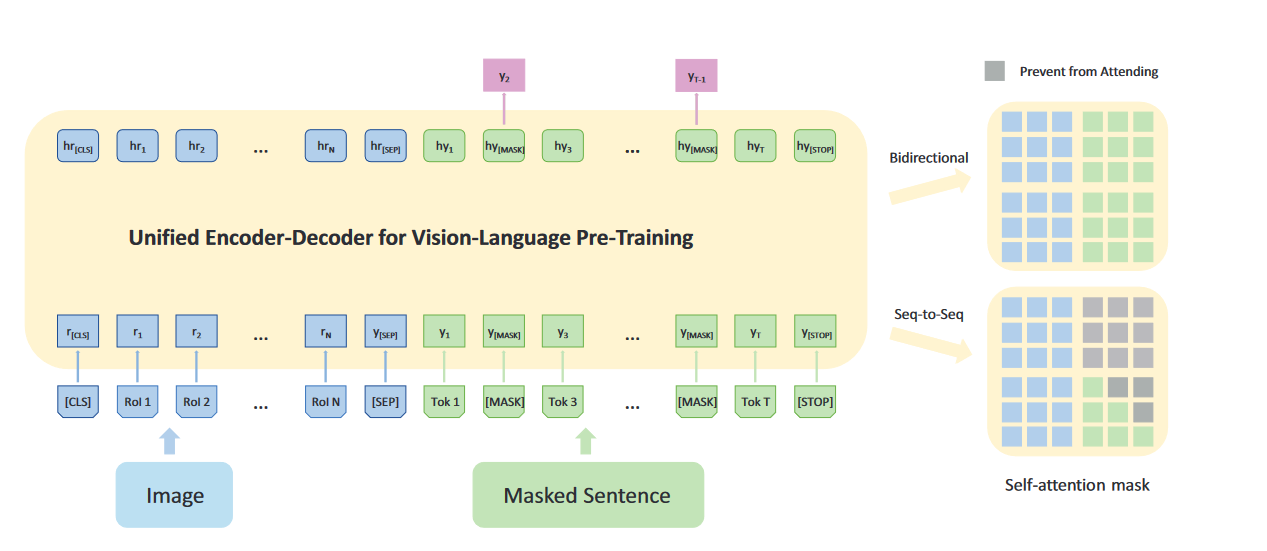
\includegraphics[scale=0.5]{image}
            \caption{预训练的模型架构。输入包括图像输入、句子输入和三个特殊标记([CLS]、[SEP]、[STOP])。图像被处理为 N 个感兴趣区域(RoIs),并根据式\ref{ri}提取区域特征。将句子标记化并用 [MASK] 标记进行掩码,以供后续掩码语言建模任务使用。我们的统一编码器-解码器由 12 层 Transformer 块组成,每个层都有一个屏蔽自注意力层和前馈模块,其中自注意力屏蔽控制预测条件的输入上下文。我们根据目标是双向还是 seq2seq 实现了两个自注意力掩码。}
            \label{procedure}
      \end{figure}


      \begin{figure}[h]
            \centering
            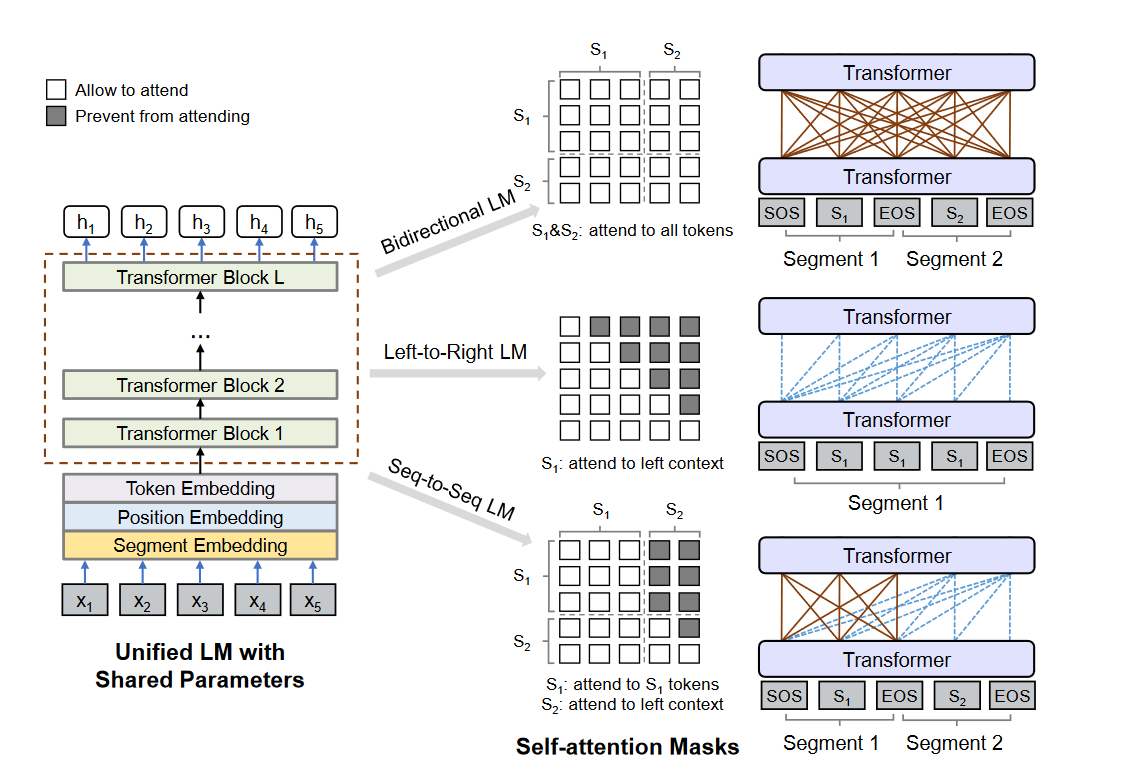
\includegraphics[scale=0.5]{uniml}
            \caption{Overview of unified LM pre-training. The model parameters are shared across the LM objectives (i.e., bidirectional LM, unidirectional LM, and sequence-to-sequence LM). We use different self-attention masks to control the access to context for each word token. }
            \label{uniml}
      \end{figure}

      为简单起见,我们假设自注意力模块中只有一个注意力头。然后,对于$H^{l-1}$的自注意力输出可以表示为:

      \begin{gather}
            V=W^l_VH^{l-1},Q=W^l_QH^{l-1},K=W^l_KH^{l-1}\\
            A^l=softmax(\frac{Q^TK}{\sqrt d}+M)V^T
      \end{gather}

      $A_l$ is further encoded by a feed-forward layer with a residual connection to form the output $H_l$


      %\newpage


      %\textit{上文的循环迭代$H_l$是由$A_l$来的吗}

      incorporating the region class probabilities ($C_i$) into region feature ($r_i$)

      %\textit{将类别与区域特征融合,这个融合是向量相加还是向量维度的增加?}

      因此,与现有工作不同,其中使用屏蔽区域预测任务来优化视觉表示,我们通过将其用于屏蔽语言重构来间接优化视觉表示。我们还选择不像BERT中那样使用下一句预测任务,或者在我们的背景下预测图像和文本之间的对应关系,因为该任务不仅比seq2seq或双向任务弱,而且计算成本高。这恰巧与RoBERTa(Liu等人,2019b年)的一项并行工作相吻合。


      \centerline{\textbf{Fine-Tuning for Downstream Tasks}}

      我们使用seq2seq目标对预训练的VLP模型在目标数据集上进行微调。在推理过程中,我们首先对图像区域进行编码,同时包括特殊的[CLS]和[SEP]标记,然后通过输入一个[MASK]标记开始生成,并从单词概率输出中抽样一个单词(例如,贪婪抽样)。然后,将前一个输入序列中的[MASK]标记替换为抽样的单词,并在输入序列中追加一个新的[MASK]标记以触发下一个预测。当选择[STOP]标记时,生成终止。其他推理方法如束搜索也可以应用。

      在微调过程中,学习了一个多层感知器(线性+ReLU+线性+Sigmoid),位于[CLS]和[SEP]的最后隐藏状态的元素级乘积之上,类似于(Lu等人,2019年)。我们使用交叉熵损失函数优化模型输出分数,相对于软答案标签。需要注意的是,与(Tan和Bansal,2019年)不同的是,在预训练期间利用了目标数据集(通过密集的人工注释),我们的预训练不需要这个要求,因此更加通用。

      \centerline{\textbf{Implementation details}}

      实现细节。我们的Transformer骨干网络与BERT-base(Devlin et al. 2018)相同。网络的输入包括图像(区域)和相关/目标标题。我们将每个输入图像表示为从Visual Genome(Krishna et al. 2017; Anderson et al. 2018)预训练的Faster RCNN的变体中提取的100个对象区域。我们将来自fc6层的模型输出作为区域特征(Ri),将1600个对象类别上的类别似然性作为区域对象标签(Ci)。值得注意的是,如果没有特别说明,我们BERT模型中的权重是从仅在文本语料库上预训练的UniLM(Dong et al. 2019)中初始化的。对于标题推断,我们在验证集上使用贪婪搜索,在测试集上使用beam search,并将beam大小设置为5。我们使用附录中呈现的配置执行轻量级模型超参数搜索。通过轻量级模型验证,将λ设置为0.75用于CC预训练(取自{0.25, 0.5, 0.75}),并将其设置为1用于图像字幕(即完全seq2seq),将其设置为0用于VQA(即完全双向)。

      模型变种和评估指标。为了展示我们的视觉语言预训练的有效性,我们首先包括一个没有这种预训练的基准模型。然后,我们包括两个极端设置的模型,其中λ =1(仅seq2seq预训练)和λ =0(仅双向预训练),以研究每个目标如何单独与不同的下游任务配合工作。我们的完整模型对两个目标进行联合训练。无论预训练配置如何,微调过程都是相同的。关于评估指标,我们对图像字幕使用标准的语言指标,包括Bleu@4、METEOR、CIDEr和SPICE,对VQA则使用官方的准确率测量,涵盖Yes/No、Number和Other等不同类型的答案。

      \section{Summary}

      本文提出了一种统一的视觉-语言预训练(VLP)模型,可以对视觉-语言生成和理解任务进行微调。该模型基于两个目标在大量图像文本对上进行了预训练:双向和seq2seq视觉-语言预测。这两个不同的目标在相同的架构下通过参数共享实现,避免了为不同类型的下游任务(即基于生成或理解的任务)需要单独的预训练模型。在我们对图像字幕和VQA任务的综合实验中,我们证明了大规模无监督的预训练可以显著加速下游任务的学习并提高模型准确性。此外,与具有单独预训练模型相比,我们的统一模型结合了从不同目标学习到的表示,并在所有下游任务上产生了稍微有所妥协但不错(SotA)的准确性。在我们的未来工作中,我们希望将VLP应用于更多的下游任务,如文本-图像对齐和视觉对话。在方法学上,我们希望看到如何将多任务微调应用于我们的框架中,以减轻不同目标之间的干扰。

      \newpage



      \section{Self-Attention}

      \begin{gather}
            Attention(Q,K,V)=softmax(\frac{QK^T}{\sqrt{d_k}})V\\
            softmax(z_i)=\frac{e^{z_i}}{\sum_{c=1}^C e^{z_c}}
      \end{gather}

      MCAN self-attention代码如下:
      \begin{lstlisting}
      # ------------------------
      # ---- Self Attention ----
      # ------------------------

      class SA(nn.Cell):
            def __init__(self, __C):
                  super(SA, self).__init__()

                  self.mhatt = MHAtt(__C)
                  self.ffn = FFN(__C)

                  self.dropout1 = nn.Dropout(p= __C.DROPOUT_R)
                  self.norm1 = nn.LayerNorm([__C.HIDDEN_SIZE])

                  self.dropout2 = nn.Dropout(p= __C.DROPOUT_R)
                  self.norm2 = nn.LayerNorm([__C.HIDDEN_SIZE])

            def construct(self, x, x_mask):
                  x = self.norm1(x + self.dropout1(
                        self.mhatt(x, x, x, x_mask)
                  ))

                  x = self.norm2(x + self.dropout2(
                        self.ffn(x)
                  ))

                  return x
      \end{lstlisting}

      当QKV都为x时,
      $$
            Attention(x,x,x)=softmax(\frac{xx^T}{\sqrt{d_x}})x
      $$
      $xx^T$:自己与自己和其他维度向量的内积矩阵。相当于x的每一维向量去与其他维度向量做点积,而向量点积又是投影积,即其他维度向量在该维向量上映射的乘积,投影值越大,说明两个向量相关性高!!!如果两个向量夹角为90°,那么说明他们没有相关性!!!

      $softmax(xx^T)$用来分配权重,看某个向量(单词)与其他维度(包括自己)的相关性强弱

      $softmax(xx^T)x$每个词的权重向量与所有词向量做内积,代表其他词向量对自身的影响(修正)

      $x$:从语料库中得到的词向量,是客观的

      $softmax(xx^T)x$:代表了上下文对每个词的修正

      再次回到QKV,
      $$
            Q=XW_Q
      $$
      可以发现,Q是由X经过线性变换得到的,$W_Q$是为了提升模型的拟合能力

      $\sqrt{d_k}$ 是为了使得方差变为1,更加稳定

      \section{Transformer}

      \begin{figure}[ht]
            \centering
            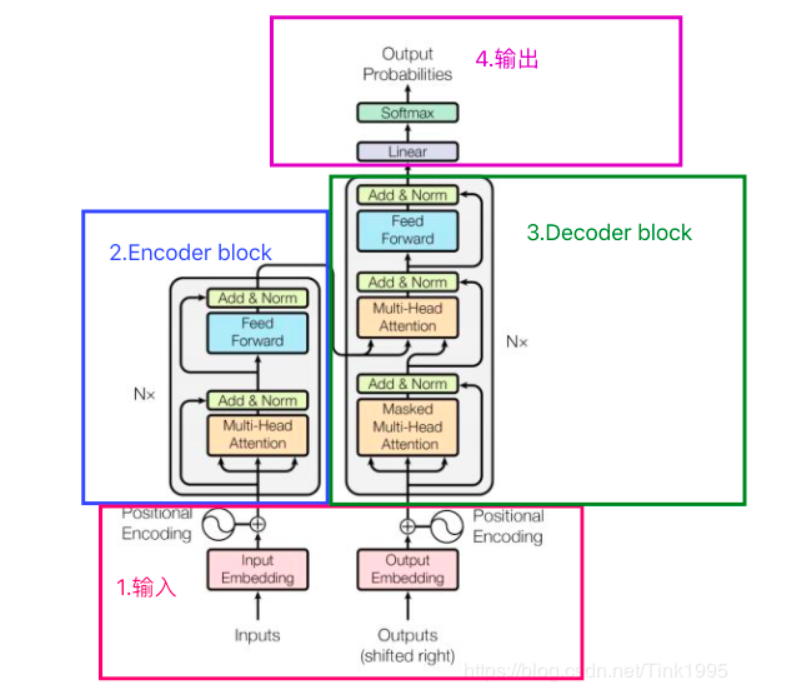
\includegraphics[scale=0.75]{transformer}
            \caption{Transformer结构图}
            \label{Transformer}
      \end{figure}

      Tokenizer和One hot都是对基础语义单元进行编码(数字化),并能体现一定语义关系

      \begin{itemize}
            \item Tokenizer给不同token分配唯一的id

                  全部token都在一维空间中表示,信息密度过于密集,语义关系表征困难
            \item One hot用二进制的每一位对应一个token

                  有多少token就有多少维度,信息密度过于稀疏,所有token之间都是正交的
      \end{itemize}

      空间变换$act2fun(X^TM+b)$:旋转拉伸+平移

      为什么涉及到维度的变换?因为在低维空间,不好把空间中的元素划分,但是升到高维,即使用简单的模型也能划分他们

      隐藏层可以代表对数据的抽象程度

      对独热向量进行降维,降维后可能每个维度的值都代表一定的语义

      \subsection{Input}
      输入是一个序列数据,可以是任意形式的词向量,但是要给每个Input Embedding层后面加上位置编码,《Attention Is All You Need》中,使用的是正余弦位置编码
      \begin{gather}
            PE(pos,2i)=\sin (\frac{pos}{1000^{\frac{2i}{d_{model}}}})\\
            \newline
            PE(pos,2i+1)=\cos (\frac{pos}{1000^{\frac{2i}{d_{model}}}})
      \end{gather}
      $d_{model}$为词向量的维度,pos 为单词的绝对位置

      选择将词向量和位置向量直接相加,而不是拼接,因为拼接的话是词向量维度翻倍

      加法是对词向量在空间中做平移操作

      为什么不选择乘法:位置对词向量影响可能盖过词向量本身

      \subsection{Enc}
      \newpage

      \begin{figure}[ht]
            \centering
            \label{enc}
            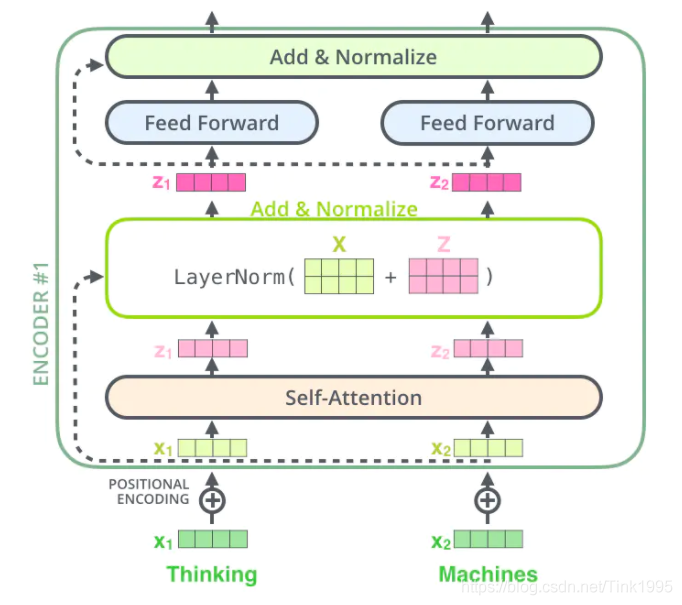
\includegraphics[scale=0.5]{enc}
            \caption{Encoder结构}
      \end{figure}
      输入的特征首先由多头机制分为多个不同的向量块,每个头负责一个向量块,每个向量块经由Self-Attention层形成一个score向量,然后再把多个头得到的scores向量拼接为与原来等大的向量,再与输入向量相加,防止神经网络退化问题,再经由一个LayerNorm与Feed Forward层,并接着引入残差,最终得到输出

      多头,每个头的输出相当于一个通道?

      \subsubsection{ResNet}

      其实就是在说
      $$
            h(x)=F(x)+x
      $$
      $F(x)$经由训练/激活函数处理后,很容易达到接近与0的水平,所以$h(x)$与$x$近似相等,就形成了恒等映射

      \subsubsection{Normalize}

      不同神经元之间进行归一化
      \begin{itemize}
            \item 提高训练速度
            \item 增加训练稳定性
      \end{itemize}


      \subsection{Dec}
      有两个输入,预测时的输入和训练时的输入。对于训练时的输入,经由一个Masked Multi-Head Attention与残差-归一化层,形成Q,然后Multi-Head Attention的K V均是Encoder层的输出
      \subsection{Output}
      首先经过一次线性变换,然后Softmax得到输出的概率分布,然后通过词典,输出概率最大的对应的单词作为我们的预测输出

      \section{BERT}

      Bidirectional Encoder Representation from Transformer


      BERT是基于上下文的模型,也就是对于同一个词,会有不同的词向量

      \newpage
      \section{Reference}

      \nocite{*} % 输出参考文献库中的所有条目

      \bibliographystyle{plain}
      \bibliography{works}

\end{sloppypar}
\end{document}